\begin{figure}[t]
\centering
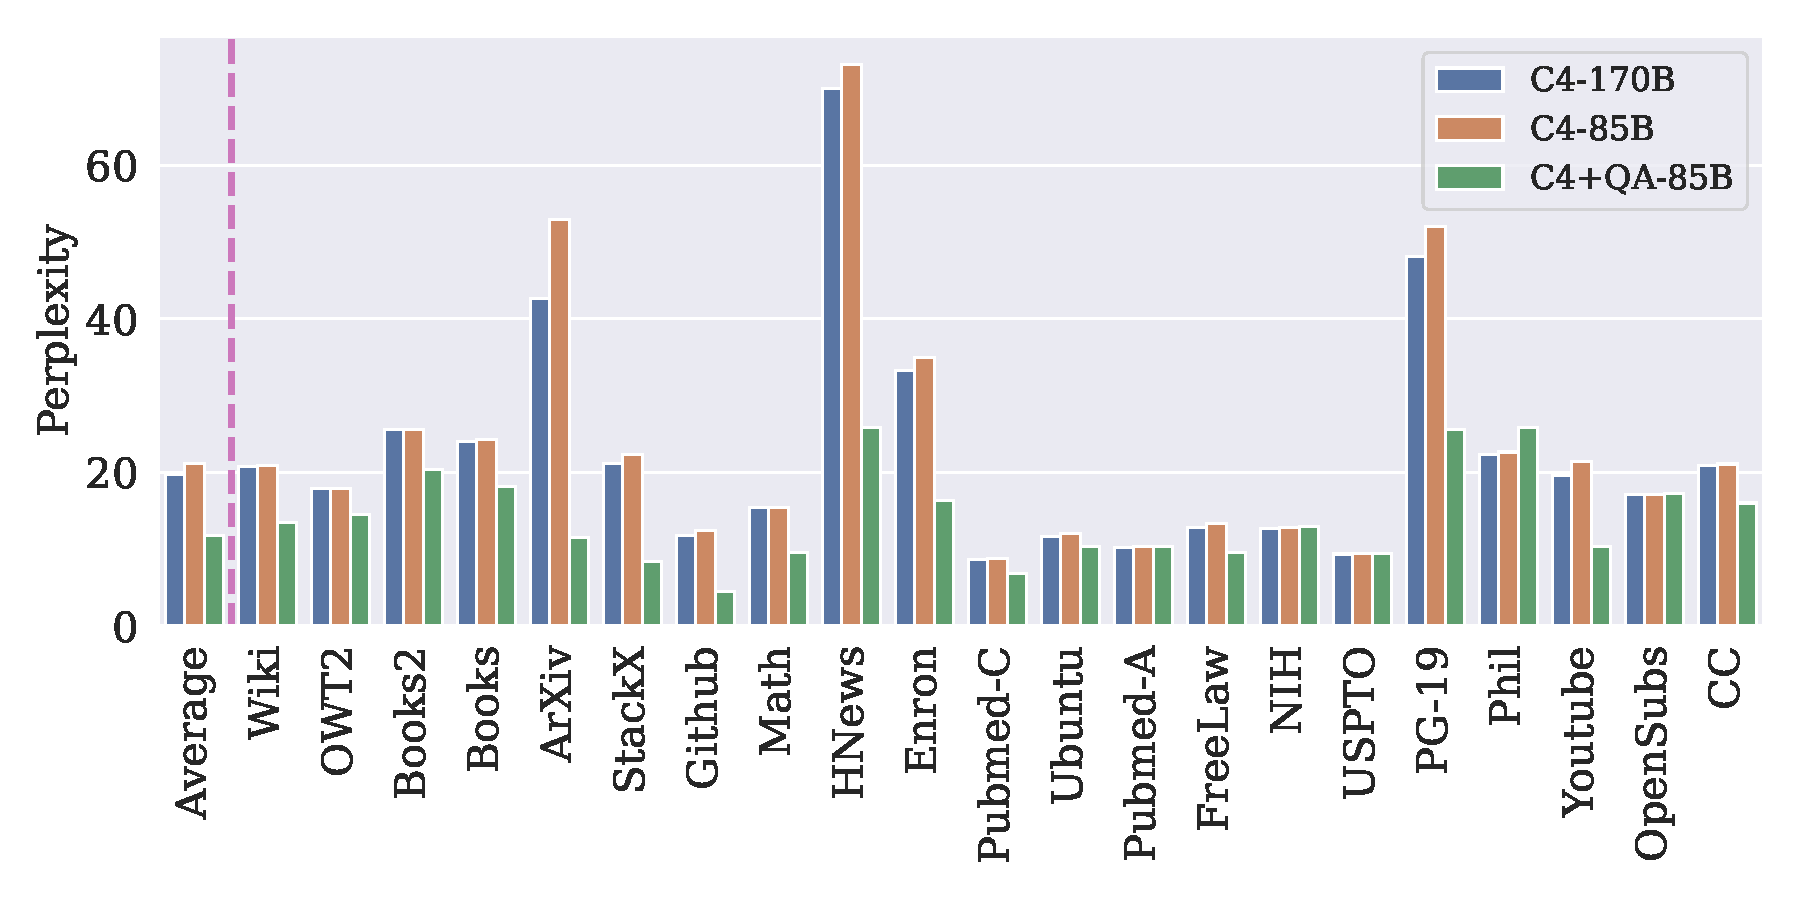
\includegraphics[width=\linewidth]{figures/all_pile_style_1.3B_300k.pdf}
\caption{\textbf{\ours~(C4 + QA-85B) v/s C4}: Comparison of perplexity on the Pile  for a 1.3B LLM trained for 300B tokens shows that WRAP outperforms models trained on 2x real data.}
\label{fig:pile_wavg}
\end{figure}


\section{Perplexity Evaluation}
\label{sec:results}






We evaluate the perplexity of the pre-trained model on the validation set of multiple out-of-distribution datasets.  
All models are either trained on the C4 dataset~\citep{raffel2020exploring}, or a particular stylistic rephrase of the same. All the evaluations are done on 21 sub-domains of the Pile~\citep{gao2020pile}.
These subsets
are created from the first 10,000 documents from each domain of the Pile dataset. We then evaluate the perplexity of the model on these subsets.  Additional evaluation details are provided in Appendix~\ref{app_eval}.
It is important to note that we evaluate perplexities on the Pile instead of C4.
Training on multiple distributions of text (synthetic and real web) does come at a small cost of less than 1 perplexity on the C4 validation set.  To understand our choice of evaluation, and why we observe this perplexity increase, we note that training over the C4 corpus corresponds to minimizing the objective 
\begin{equation}
    \theta_{c4}   = \min_{\theta} \mathbb{E}_{x \sim D_{c4}}\left[ \mathcal{L}(\theta; x) \right], 
    \label{eq:theta}
\end{equation}
that attempts to exactly model the C4 web text.  In contrast, training over multiple styles corresponds to minimizing the risk over a different distribution,

\begin{equation}
    \theta_{\ours}   = \min_{\theta} \mathbb{E}_{x \sim D_{c4}\cup D_{syn}}\left[ \mathcal{L}(\theta; x) \right] .
    \label{eq:theta_syn}
\end{equation}

Solving for \eqref{eq:theta_syn} does not minimize the risk over C4-only, and hence it is unfair to compare
$\theta_{c4}$ and
$\theta_{\ours}$ on the C4.
For meaningfully comparing models trained on the C4 and on its synthetic rephrases, we evaluate their generalization capability on 21 different domains of the Pile~\citep{gao2020pile}. 
Results for each domain are presented in Figure~\ref{fig:pile_wavg}.




\paragraph{Data Complexity}
In Figure~\ref{fig:lower_right_image}, we show that models trained for fewer tokens (150B) and even smaller 350M models outperform training on the full C4 for 300B tokens indicating faster learning with synthetic rephrases.  
On some domains such as ArXiv and HackerNews, we observe that training with synthetic data allows reducing the perplexity by nearly 3x of the perplexity of models trained on real data alone. This suggests that in many cases 
it may not be possible to offset 
the performance advantage of pre-training on synthetic data
by merely training on more real data.
Overall, on an average of multiple subsets of the Pile,
our models improve perplexity by 50\% over models trained on real data alone. 

\paragraph{Learning Speed}
We observe that even at the first checkpoint (10B tokens) of \ours~training, the average perplexity of the LLM on the Pile is lower than that achieved by pre-training on C4 for 15 checkpoints. This suggests a 15x pre-training speed-up. We defer the discussion on learning speed to  `zero-shot' tasks in order to make more meaningful comparisons. 






\section{Zero-shot Tasks}
We now evaluate our pre-trained language models on various zero-shot question answering (QA) benchmarks
using the LLM Evaluation Harness\footnote{We use git commit - \texttt{89618bf8} for consistency across all experiments with a batch size of 32.}~\citep{eval-harness}.

\subsection{Datasets}
We evaluate our models on a total of 13 different zero-shot benchmarks to assess their abilities across various natural language tasks like common sense reasoning, language and knowledge understanding and mathematical reasoning.

\paragraph{General Understanding}
The General Understanding category comprises datasets testing broader cognitive skills and language comprehension. \textbf{ARC Easy (ARC-E)}~\citep{allenai:arc} is the less challenging counterpart of ARC-C, featuring questions that require basic reasoning skills. \textbf{BoolQ}~\citep{clark-etal-2019-boolq} includes boolean questions that focus on reading comprehension and general language understanding. \textbf{Winogrande (Wino.)}~\citep{ai2:winogrande} challenges models with common sense reasoning in language, particularly in pronoun disambiguation. \textbf{PIQA}~\citep{Bisk2020} assesses understanding of physical processes, an essential part of practical common sense. \textbf{HellaSwag}~\citep{zellers2019hellaswag} tests the ability to complete scenarios coherently, demanding both language understanding and common sense. \textbf{TruthfulQA}~\citep{lin2021truthfulqa} is centered on generating truthful, accurate answers, thus testing the model's factual correctness. \textbf{OpenBookQA (OBQA)}~\citep{OpenBookQA2018} evaluates the understanding of a broad range of facts and concepts. Finally, \textbf{LogiQA-2}~\citep{logiqa2} assesses the model's capacity to comprehend and apply logical principles.

\paragraph{Specialized Knowledge}
In the Specialized Knowledge category, we include datasets that demand expertise in specific domains. The \textbf{ARC Challenge (ARC-C)}~\citep{allenai:arc} contains challenging science exam questions from grades 3 to 9, demanding advanced knowledge. \textbf{SciQ}~\citep{SciQ} provides science exam questions to test models' understanding and reasoning in the scientific domain. \textbf{PubMedQA}~\citep{jin2019pubmedqa} focuses on biomedical literature, assessing comprehension in medical and health-related information. 
\textbf{MathQA}~\citep{amini-etal-2019-mathqa} tests mathematical problem-solving, requiring both numerical comprehension and reasoning. Lastly, \textbf{MMLU}~\citep{hendryckstest2021} spans multiple domains, from professional to academic, testing the model on specialized subjects.





\begin{table*}[t]
    \centering
    \scalebox{0.8}{
    \begin{tabular}{lcccccccc>{\columncolor{LightCyan}}c}
        \toprule
        Dataset (Real Tok.) & ARC-E & BoolQ & Wino. & PIQA & HellaSwag & TruthfulQA & OBQA & LogiQA & Avg \\
        \midrule
        Half C4 (85B) & 61.2  &  59.1  &  57.3  &  74.9  &  46.5  &  34.1  &  22.4  &  23.5  &  47.4 \\
        Full C4 (170B) & 61.6  &  54.2  &  59.0  &  74.9  &  46.8  &  33.5  &  25.0  &  23.4  &  47.3 \\
        RW (160B) &  61.6  &  60.7  &  57.5  &  74.3  &  45.2  &  36.8  &  21.8  &  23.2  &  47.6 \\
        RW (320B) & 60.7  &  61.1  &  57.1  &  74.4  &  45.6  &  36.0  &  22.6  &  22.5  &  47.5 \\
        Pythia-Pile (300B) &   60.5  &  63.3  &  57.5  &  70.8  &  40.4  &  38.9  &  22.2  &  22.2  &  47.0 \\
        TinyLlama (1T) & 60.3  &  57.8  &  59.1  &  73.3  &  45.0  &  37.6  &  21.8  &  24.5  &  47.4 \\
        \midrule
        Synthetic (85B) &63.9  &  60.0  &  58.8  &  76.1  &  45.2  &  44.0  &  23.0  &  24.1  &  49.4\\
        Synthetic+C4 (85B) & 64.1  &  62.2  &  58.9  &  75.4  &  46.2 &  40.6  &  24.1  &  23.9  &  49.4 \\
        \bottomrule
    \end{tabular}}
    \caption{Evaluation of $\sim1.3$B parameter LLMs on `General Understanding Tasks'  on datasets focusing on general reasoning, language understanding, and common sense. Results for \ours are averaged over 3 runs}
    \label{tab:general_understanding}
\end{table*}


\begin{table*}[t]
    \centering
    \scalebox{0.8}{
    \begin{tabular}{lccccc>{\columncolor{LightCyan}}c}
        \toprule
        Dataset (Real Tok.) & ARC-C & SciQ & PubMedQA & MathQA & MMLU & Avg \\
        \midrule
        Half C4 (85B) & 26.3  &  84.5  &  57.2  &  23.4  &  24.2  &  43.1 \\
        Full C4 (170B) & 26.8  &  85.0  &  57.4  &  24.3  &  23.9  &  43.5 \\
        RW (160B) & 27.2  &  87.2  &  56.2  &  24.1  &  25.9  &  44.1 \\
        RW (320B) & 27.8  &  88.0  &  57.4  &  23.0  &  25.4  &  44.3 \\
        Pythia-Pile (300B) &  26.1  &  86.6  &  60.6  &  25.2  &  24.3  &  44.6 \\
        TinyLlama (1T) & 27.8  &  88.9  &  61.4  &  24.1  &  25.8  &  45.6 \\
        \midrule
        Synthetic (85B) & 29.7  &  87.0  &  60.2  &  23.4  &  24.6  &  45.0 \\
        Synthetic+C4 (85B) & 29.9  &  87.6  &  61.5  &  23.9  &  24.8  &  45.5 \\
        \bottomrule
    \end{tabular}}
    \caption{Evaluation of $\sim1.3$B parameter LLMs on `Specialized Knowledge Tasks'  that require specific domain knowledge such as science, medicine, mathematics, and logic. Results for \ours are averaged over 3 runs.}
    \label{tab:specialized_knowledge}
\end{table*}

\subsection{Results}
We compare the performance of a model trained on a mixture of real and synthetic data with models trained on various splits of real data. In all our experiments, we use the C4~\citep{raffel2020exploring} dataset for rephrasing and producing splits of synthetic data. 
We use the abbreviation `Real Tok.' to denote the number of tokens of web data available for pre-training. In the `Synthetic + Real' experiments, we augment the same number of synthetic rephrases. We choose `Real Tokens' as the metric of comparison because we can potentially rephrase the same document multiple times, implying that the total corpus size is not meaningful, and corpus `knowledge' is the actual currency of interest.

\paragraph{Baselines Methods}
We pre-train LLMs of 
(i) Half of C4, and the (ii) Full C4 corresponding to approximately
85 Billion and 170 Billion real tokens respectively~\citep{raffel2020exploring}. We also pre-train our own models on (iii) 160 Billion and (iv) 320 Billion tokens of the RefinedWeb Dataset~\citep{penedo2023refinedweb}. Additionally, we also compare with the (iv) Pythia-1.4B model that was trained on the Pile~\citep{gao2020pile}. This dataset is no longer publicly available, hence we utilize a pre-trained model. Finally, we also compare with the recent (v) TinyLlama model~\citep{zhang2024tinyllama} that was trained for 3 epochs  on 1 Trillion tokens of data from 
SlimPajama \citep{shen2023slimpajama} and StarCoder \citep{li2023starcoder}.


\paragraph{General Improvements}
Across all tasks in Table~\ref{tab:general_understanding}, we observe that models trained on synthetic data combined with the C4 dataset (Synthetic+C4) exhibit an overall higher average performance of 49.4\% as compared to those trained solely on the real C4 dataset with a 85B token split, which scored an average of 47.4\%. This shows that the inclusion of synthetic data can enhance the general understanding capabilities of NLP models. Moreover, even the TinyLLama model trained for 10x compute and data, performs comparably to the other models trained on real data. This suggests that the gains from filtering out, or adding more real data are very low. As opposed to this, \ours~shows that pre-training on even small amounts of synthetic data can contribute to large performance gains.

\paragraph{Specialized Knowledge Tasks} 
The key message from the results
in Table~\ref{tab:specialized_knowledge} is that synthetic data can not impart `new knowledge'. It can only help pre-train faster, which was also the premise of our work. In particular, we note several key findings:
\begin{enumerate}
    \item Pre-training on larger datasets helps improve performance, by presumably exposing the LLM to more ``knowledge''. For instance, the Pythia (300B) model achieves an average score of 44.6\%, outperforming the smaller C4 (85B) dataset's score of 43.5\%.
    \item Despite the advantages of a larger dataset, the improvements saturate. For example, RefinedWeb (320B) model outperforms the RefinedWeb (160B) model by only 0.2\%. Similarly, the TinyLlama model (1T tokens) performs comparably to the \ours~ model, which only had 85B tokens of raw web data.
\end{enumerate}

\paragraph{Specific Improvements} 
We see maximum improvement in the TruthfulQA dataset, with the Synthetic (85B) model scoring 44.0\%, which is significantly higher than any other model's performance on this dataset. This is potentially because instruction-tuned LLMs already correct potential misconceptions while rephrasing the text. Interestingly, we notice how adding real data to the synthetic model (Synthetic+C4) reduces the performance on TruthfulQA by 4\%, down to 40.5\%, indicating a potential dilution of the benefits gained from synthetic data when combined with real data. Other datasets such as HellaSwag, and BoolQ, for which C4 trained models do well, continue to show the benefits of incorporating combinations of C4 and synthetic rephrases.

